%% For double-blind review submission, w/o CCS and ACM Reference (max submission space)
\documentclass[sigplan]{acmart}
\settopmatter{printfolios=true,printccs=false,printacmref=false}
\settopmatter{printacmref=false} % Removes citation information below abstract
\renewcommand\footnotetextcopyrightpermission[1]{} % removes footnote with conference information in first column
\pagestyle{plain} % removes running headers

\acmJournal{PACMPL}
\acmVolume{1}
\acmNumber{POPL} % CONF = POPL or ICFP or OOPSLA
\acmArticle{1}
\acmYear{2019}
\acmMonth{1}
\acmDOI{} % \acmDOI{10.1145/nnnnnnn.nnnnnnn}
\startPage{1}

%% Copyright information
%% Supplied to authors (based on authors' rights management selection;
%% see authors.acm.org) by publisher for camera-ready submission;
%% use 'none' for review submission.
\setcopyright{none}
%\setcopyright{acmcopyright}
%\setcopyright{acmlicensed}
%\setcopyright{rightsretained}
%\copyrightyear{2018}           %% If different from \acmYear

%% Bibliography style
\bibliographystyle{ACM-Reference-Format}
%% Citation style
%% Note: author/year citations are required for papers published as an
%% issue of PACMPL.
\citestyle{acmauthoryear}   %% For author/year citations


\usepackage{url}
\usepackage{amsmath}
\usepackage{amsfonts}
\usepackage{amssymb}
\usepackage{listings}
\usepackage{color}
\usepackage{graphicx}

%% https://github.com/nickgian/thesis/blob/master/lstcoq.sty
\usepackage{color}

\definecolor{ltblue}{rgb}{0,0.4,0.4}
\definecolor{dkblue}{rgb}{0,0.1,0.6}
\definecolor{dkgreen}{rgb}{0,0.35,0}
\definecolor{dkviolet}{rgb}{0.3,0,0.5}
\definecolor{dkred}{rgb}{0.5,0,0}

% lstlisting coq style (inspired from a file of Assia Mahboubi)
%
\lstdefinelanguage{Coq}{ 
%
% Anything betweeen $ becomes LaTeX math mode
mathescape=true,
%
% Comments may or not include Latex commands
texcl=false, 
%
% Vernacular commands
morekeywords=[1]{Section, Module, End, Require, Import, Export,
  Variable, Variables, Parameter, Parameters, Axiom, Hypothesis,
  Hypotheses, Notation, Local, Tactic, Reserved, Scope, Open, Close,
  Bind, Delimit, Definition, Let, Ltac, Fixpoint, CoFixpoint, Add,
  Morphism, Relation, Implicit, Arguments, Unset, Contextual,
  Strict, Prenex, Implicits, Inductive, CoInductive, Record,
  Structure, Canonical, Coercion, Context, Class, Global, Instance,
  Program, Infix, Theorem, Lemma, Corollary, Proposition, Fact,
  Remark, Example, Proof, Goal, Save, Qed, Defined, Hint, Resolve,
  Rewrite, View, Search, Show, Print, Printing, All, Eval, Check,
  Projections, inside, outside, Def},
%
% Gallina
morekeywords=[2]{forall, exists, exists2, fun, fix, cofix, struct,
  match, with, end, as, in, return, let, if, is, then, else, for, of,
  nosimpl, when},
%
% Sorts
morekeywords=[3]{Type, Prop, Set, true, false, option},
%
% Various tactics, some are std Coq subsumed by ssr, for the manual purpose
morekeywords=[4]{pose, set, move, case, elim, apply, clear, hnf,
  intro, intros, generalize, rename, pattern, after, destruct,
  induction, using, refine, inversion, injection, rewrite, setoid_rewrite, congr,
  unlock, compute, ring, field, fourier, replace, setoid_replace, fold, unfold,
  change, cutrewrite, simpl, have, suff, wlog, suffices, without,
  loss, nat_norm, assert, cut, trivial, revert, bool_congr, nat_congr,
  symmetry, transitivity, auto, split, left, right, autorewrite},
%
% Terminators
morekeywords=[5]{by, done, exact, reflexivity, tauto, romega, omega,
  assumption, solve, contradiction, discriminate},
%
% Control
morekeywords=[6]{do, last, first, try, idtac, repeat},
%
% Comments delimiters, we do turn this off for the manual
morecomment=[s]{(*}{*)},
%
% Spaces are not displayed as a special character
showstringspaces=false,
%
% String delimiters
morestring=[b]",
morestring=[d]’,
%
% Size of tabulations
tabsize=3,
%
% Enables ASCII chars 128 to 255
extendedchars=false,
%
% Case sensitivity
sensitive=true,
%
% Automatic breaking of long lines
breaklines=false,
%
% Default style fors listings
basicstyle=\small,
%
% Position of captions is bottom
captionpos=b,
%
% flexible columns
basewidth={2em, 0.5em},
columns=flexible,
%
% Style for (listings') identifiers
identifierstyle={\ttfamily\color{black}},
% Style for declaration keywords
keywordstyle=[1]{\ttfamily\bfseries\color{dkviolet}},
% Style for gallina keywords
keywordstyle=[2]{\ttfamily\bfseries\color{dkgreen}},
% Style for sorts keywords
keywordstyle=[3]{\ttfamily\bfseries\color{ltblue}},
% Style for tactics keywords
keywordstyle=[4]{\ttfamily\color{dkblue}},
% Style for terminators keywords
keywordstyle=[5]{\ttfamily\color{dkred}},
%Style for iterators
%keywordstyle=[6]{\ttfamily\color{dkpink}},
% Style for strings
stringstyle=\ttfamily,
% Style for comments
commentstyle={\ttfamily\itshape\color{dkgreen}},
%
%moredelim=**[is][\ttfamily\color{red}]{/&}{&/},
literate=
    {fun}{{\color{dkgreen}{$\lambda\;$}}}1
    {bool}{{$\mathbb{B}$}}1
    {nat}{{$\mathbb{N}$}}1
    {Vforall2}{Vforall2}1 % quick workardoun to avoid partial replacement of 'forall' in identifier
    {nat\_equiv}{nat\_equiv}1 % quick workardoun to avoid partial replacement of 'nat' in identifier
    {forall}{{\color{dkgreen}{$\forall\;$}}}1
    {exists}{{$\exists\;$}}1
    {<-}{{$\leftarrow\;\;$}}1
    {=>}{{$\Rightarrow\;\;$}}1
    {==}{{\texttt{==}\;}}1
    {==>}{{$\Longrightarrow\;\;$}}1
%    {:>}{{\texttt{:>}\;}}1
    {->}{{$\rightarrow\;\;$}}1
    {<-->}{{$\longleftrightarrow\;\;$}}1
    {<->}{{$\leftrightarrow\;\;$}}1
    {<==}{{$\leq\;\;$}}1
    {\#}{{$^\star$}}1 
    {\\o}{{$\circ\;$}}1 
%    {\@}{{$\cdot$}}1 
    {\/\\}{{$\wedge\;$}}1
    {\\\/}{{$\vee\;$}}1
    {++}{{\texttt{++}}}1
    {~}{{\ }}1
    {¬}{{$\lnot$}}1     % this does not work
    {\@\@}{{$@$}}1
    {\\mapsto}{{$\mapsto\;$}}1
    {\\hline}{{\rule{\linewidth}{0.5pt}}}1
%
}[keywords,comments,strings]

\lstnewenvironment{coq}{\lstset{language=Coq}}{}

% pour inliner dans le texte
\def\coqe{\lstinline[language=Coq, basicstyle=\small]}
% pour inliner dans les tableaux / displaymath...
\def\coqes{\lstinline[language=Coq, basicstyle=\scriptsize]}

%%% Local Variables: 
%%% mode: latex
%%% Local IspellDict: british
%%% TeX-master: "main.tex"
%%% End: 
%\usepackage{booktabs}   %% For formal tables:
%\usepackage{subcaption}

\newcommand{\N}{\mathbb{N}}
\newcommand{\Z}{\mathbb{Z}}
\newcommand{\bool}{\mathbb{B}}

\begin{document}

%% Title information
\title{Formal verification of floating-point numbers conversion between ASN.1 BER and IEEE 754 binary encodings}
%\subtitle{Subtitle}

\author{Ilia Zaichuk}
\affiliation{
  \institution{Digamma.ai}
}
\email{izaichuk@digamma.ai}

\author{Vadim Zaliva}
\affiliation{
  \institution{CMU, Digamma.ai}
}
\email{lord@digamma.ai}

\begin{abstract}

ASN.1 encoding is widely used for data transfer between various computing systems.
Such data may contain floating-point numbers. The most common representation of floating-point
numbers is IEEE 754 standard. ASN.1, however, does not rely
on IEEE for that task. Conversion between IEEE and ASN.1 floating-point
representations is error-prone in most ASN.1 protocol implementations. In this
project, we set to formalize such conversion and prove it's correctness using the Coq proof assistant.
Such formalization could be used as ``executable specification'' which could be
extracted as an OCaml or Haskell program. The secondary goal of this project is
to asses the amount of work required for formalizing the full ASN.1 stack, which
we are considering as the next step.

\end{abstract}


%% \maketitle
\maketitle



\section{Introduction}

At the fundamental level, any floating-point number is a pair of integers: a \textit{mantissa} (sometimes also called \textit{significand}) and an \textit{exponent}. The main difference between the various standards for floating-point representations is how this pair is encoded. Different binary lengths might be used, different representations for special values might be chosen. These variations in encoding are adapted for various use-cases but create complications when conversion from one format to another is required.

An instance of this, which is handled in our project, is the conversion between floating-point numbers, encoded in IEEE 754 and ASN.1 formats. It is a common task, but that does not make it a simple one. Mere numbers: while any IEEE encoding consists of 3 different parts. An ASN.1 float has at least 9.

To give you an example, in the \emph{asn1c} \cite{walkinopen} project, the function
converting between the two formats takes up around 200 lines of C code.
It is quite hard
for a human to verify, making a formalization of the topic a much-needed endeavor.

\section{Brief format comparison}

In the scope of this project, two formats are considered: the IEEE 754 binary
interchange floating-point encoding \cite{5976968} and the ASN.1 BER real value encoding \cite{ISO8825}.
IEEE 754 defines formats of varying lengths, \emph{binary32} and \emph{binary64}
being the most commonly used. Any IEEE 754 floating-point
number can be thought of as a triplet:
$(\mathrm{sign}, \mathrm{exp}, \mathrm{mantissa}) \in \bool \times \Z \times \N$,
which is serialized as concatenation of bit sequences representing each of the components.

The core part of any ASN.1 real encoding has the following form:
$ (\mathrm{sign},\mathrm{radix},\mathrm{scaling},\mathrm{exp},\mathrm{mantissa})
\in \bool \times \N \times \N \times \Z \times \N$.
The serialization scheme is more complicated, using additional
information about the encoding variants.

Both standards define more than one encoding scheme, but for the purposes of
this project, only binary formats are considered: those, in which the exponent using a base which is power of two. In addition to real values, the standards support the same set(s)
of special values, however, an
IEEE \emph{NaN} value must lose its debugging payload when conversion to
ASN.1 is performed.

While consisting of blocks of similar meaning, ASN.1 and IEEE 754 represent same numbers in different ways. For example, the number $0.46875 = 15*2^{-5}$ corresponds to the $(0, 125, 7340032)$ tuple in IEEE binary32, and $(0, 16, 2, 254, 29)$ ASN.1 real  encoding.

It is important to note that any number in binary128, 64 or 32 IEEE format can
be converted to ASN.1 without loss of precision. Conversely, an ASN.1-encoded
number is not necessarily representable in any common IEEE format. For such cases
rounding is implemented, discussed in Section~\ref{sec:imp}.

\section{Implementation}
\label{sec:imp}
\begin{figure}[h!]
  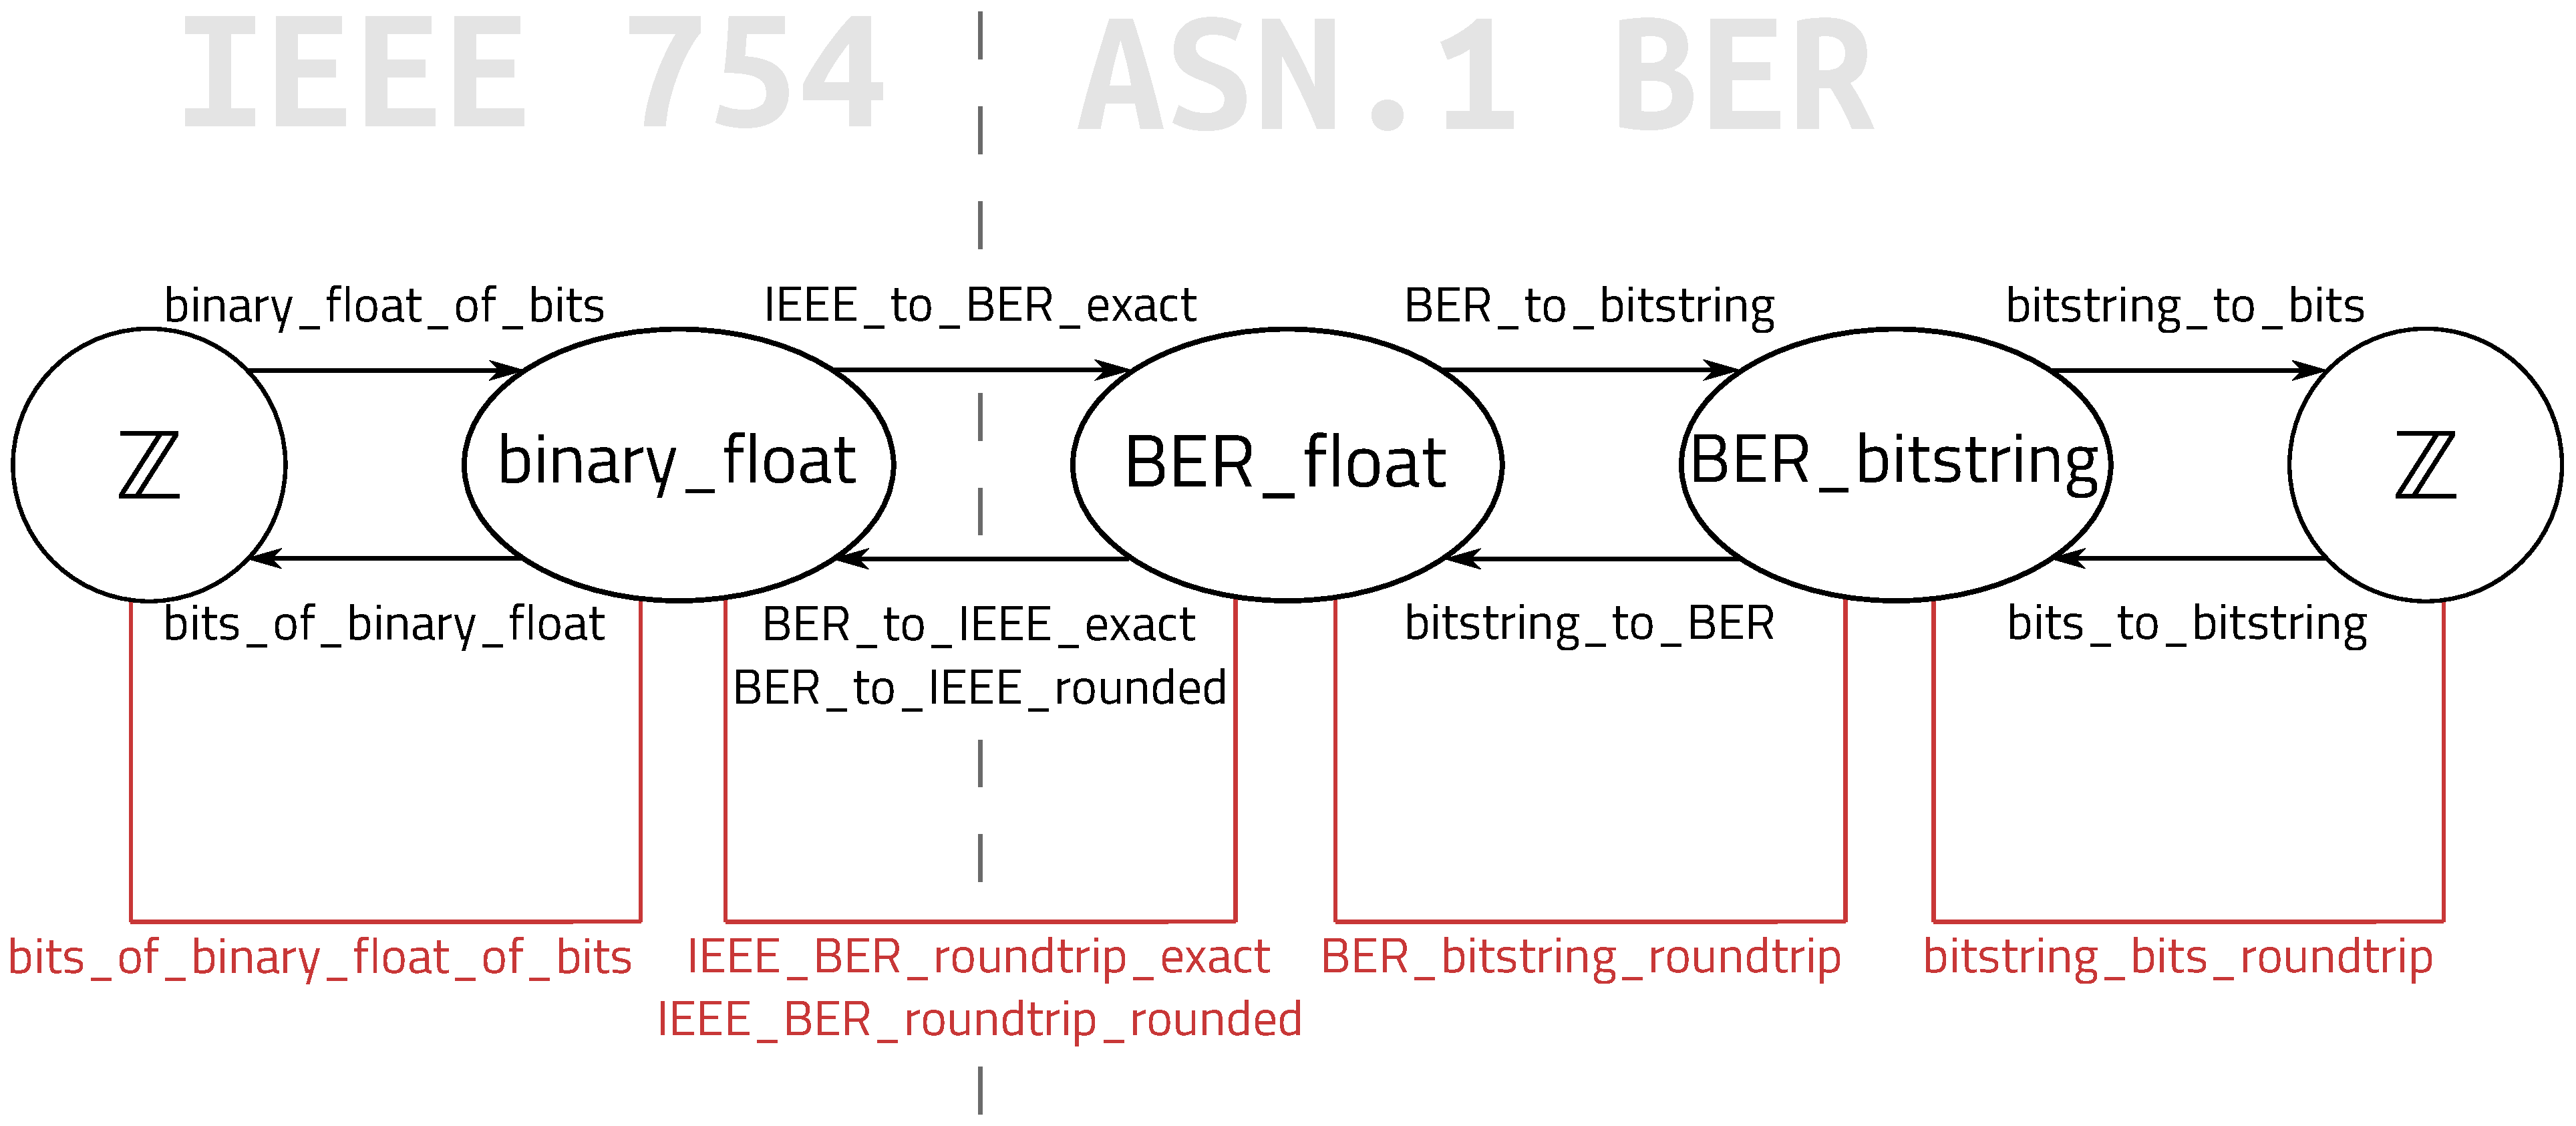
\includegraphics[width=\columnwidth]{diagram.eps}
  \caption{Full conversion scheme}
  \label{fig:figure1}
\end{figure}

The conversion path is shown on Figure~\ref{fig:figure1}. We use $\Z$ to
represent bit strings or arbitrary length. Both BER and IEEE floating-point
numbers are ultimately encoded as such strings. The conversion is split into
several steps with intermediate representations. On IEEE side there is
binary\_float, defined in the Flocq \cite{boldo2011flocq} library which provides
an abstract representation of floats as an inductive type with constructors for
special values as well as ``regular'' numbers expressed as a mantissa-exponent
pair. On ASN.1 side, there is the BER\_float inductive type, which is similar
to binary\_float, with some additional parameters unique to BER added, and the BER\_bitstring type, which is used as an intermediate type for generating sequence of bits.

For each adjacent pair of formats we need to define two conversion functions
(for both directions), a heterogeneous equality, and lemmas ensuring equivalence
of conversion results in both directions.

In general, our conversion function from type $T$ to $U$ is not total.
The converter may fail for some values of $T$ which could not be
represented in $U$. To express this, our
convertors have the type $T \rightarrow \mathrm{option}\, U$, using the
\emph{Option Monad}. In case of error \emph{None} is returned.
This allows us to define a generic ``round-trip'' conversion correctness property as follows:

\begin{lstlisting}[language=Coq, mathescape=true,
  basicstyle=\footnotesize]
Definition roundtrip
           (A1 B A2 : Type)
           (f : A1 -> option B) (* forward pass *)
           (b : B -> option A2) (* backward pass *)
           (e : A1 -> A2 -> bool)   (* equality *)
           (x : A1)            (* value *)
  : Prop :=
    is_Some_b (f x) = true ->
    bool_het_inverse option A1 B A2 f b e x = Some true.
\end{lstlisting}

The original expression of type $A1$ is converted using ``forward'' conversion
pass to type $B$, and then back using ``backward'' pass to type $A1$. For example, a practical scenario for this could be encoding ($f$) a \emph{binary32} ($A1$) float in BER ($B$), transmitting it over a network, and decoding ($b$) into \emph{binary64} ($A2$). The results
of successful forward conversion must satisfy a heterogeneous equality
predicate \emph{e}, which is applied using  \emph{bool\_het\_inverse} wrapper:

\begin{lstlisting}[language=Coq, mathescape=true,
  basicstyle=\footnotesize]
Definition bo$$ol_het_inverse
  (m : Type -> Type) `{Monad m}
  (A1 B A2 : Type)
  (f : A1 -> m B)  (b : B -> m A2)
  (e : A1 -> A2 -> bool) (x : A1) : m bool := 
  y <- f x ;;
    x' <- b y ;;
      ret (e x x').
\end{lstlisting}

It should be noted that, while we call it a ``roundtrip'', the result
of the backwards pass ($A2$) does not have the same type as the original value ($A1$).
The reason for this is the need to convert between different formats of IEEE 754: for
example, a \emph{binary64} floating-point number might be transmitted, using BER format,
to a different machine, where it needs to be represented in \emph{binary32}.
In such cases rounding might need to be performed during conversion from BER to IEEE.
This is supported in our implementation, with the the roundtrip conversion behaving exactly as if the
original number was converted to a different format according to the rules set out in
IEEE 754.

For the common IEEE 754 binary formats, high-level encoding end decoding functions were defined. For example for \emph{binary64}:

\begin{lstlisting}[language=Coq, mathescape=true,
  basicstyle=\footnotesize]
    Definition float64_to_BER_exact (f : Z) : option Z :=
      ab <- b64_to_BER_abstract (b64_of_bits f) ;;
        ret (BER_to_bits ab).

    Definition BER_to_float64_exact (asn : Z) : option Z :=
      bf <- bits_to_BER asn ;;
        af <- BER_to_b64_abstract_exact bf ;;
          ret (bits_of_b64 af).

    Definition BER_to_float64_rounded
      (rounding : mode ) (asn : Z) : option Z :=
        bf <- bits_to_BER asn ;;
          af <- BER_to_b64_abstract_rounded rounding bf ;;
            ret (bits_of_b64 af).
\end{lstlisting}

The implementation is straightforward. It proceeds by converting a bit string in
source format into the target one through intermediate steps corresponding to
intermediate formats that we introduced. If an error occurs at any step
(\emph{None} returned) it is propagated to the final result through
monadic composition of the steps.

\section{Results and Future work}

To demonstrate how our verified implementation could be used in practical ASN.1 encoding/decoding pipeline, we exported our encoder and decoder implementation in Gallina as OCaml program using Coq \textit{extraction}\cite{letouzey2008extraction} facility. 

The resulting implementation was then linked to asn1c library, replacing native implementation of floating point encoding module. It was then tested to pass all unit tests. The performance of the extracted code is, as expected, is slower compared to original C implementation.

To combine benefits of formal verification with high performance of native
implementation we plan as the next step to try to verify existing C implementation
using our formalization as the specification. We are considering using
VST\cite{appel2011verified} and the CompCert compiler\cite{leroy2012compcert}. 

The ultimate goal is to verify the full ASN.1 stack. This is a formidable task as
ASN.1 specification is very rich and includes multiple encoding formats
(binary, XML, etc.) and even it's own embedded constraints language. We are
seeking industrial and academic partners to work with us on this project.

\nocite{*}
\bibliography{paper}

\end{document}